
% ----------------------------------------------------------------------
%  Set the document class
% ----------------------------------------------------------------------
\documentclass[11pt,a4paper,twoside]{article}

% ----------------------------------------------------------------------
% Define external packages, language, margins, fonts and new commands
% ----------------------------------------------------------------------
%\input{preamble} 
\usepackage[utf8]{inputenc}   % <<<<< Linux
\usepackage[english]{babel} % <<<<< English
\usepackage{notoccite}
\usepackage[skip=0.5\baselineskip]{caption}
\hyphenation{GTKWave}
\usepackage{listings}
\usepackage[all]{nowidow}

%blind text
\usepackage{lipsum}

\usepackage{graphicx}
\graphicspath{{./}{../../figlib/}{../mat/}{../sim/}}
\def\FontLn{% 16 pt normal
  \usefont{T1}{phv}{m}{n}\fontsize{16pt}{16pt}\selectfont}
\def\FontLb{% 16 pt bold
  \usefont{T1}{phv}{b}{n}\fontsize{16pt}{16pt}\selectfont}
\def\FontMn{% 14 pt normal
  \usefont{T1}{phv}{m}{n}\fontsize{14pt}{14pt}\selectfont}
\def\FontMb{% 14 pt bold
  \usefont{T1}{phv}{b}{n}\fontsize{14pt}{14pt}\selectfont}
\def\FontSn{% 12 pt normal
  \usefont{T1}{phv}{m}{n}\fontsize{12pt}{12pt}\selectfont}

% Use Arial font as default
%
\renewcommand{\rmdefault}{phv}
\renewcommand{\sfdefault}{phv}
\usepackage{geometry}	
\geometry{verbose,tmargin=2.5cm,bmargin=2.5cm,lmargin=2.5cm,rmargin=2.5cm}

%\usepackage{setspace}
%\renewcommand{\baselinestretch}{1.5}

\usepackage[pdftex]{hyperref} % enhance documents that are to be
                              % output as HTML and PDF
\hypersetup{colorlinks,       % color text of links and anchors,
                              % eliminates borders around links
%            linkcolor=red,    % color for normal internal links
            linkcolor=black,  % color for normal internal links
            anchorcolor=black,% color for anchor text
%            citecolor=green,  % color for bibliographical citations
            citecolor=black,  % color for bibliographical citations
%            filecolor=magenta,% color for URLs which open local files
            filecolor=black,  % color for URLs which open local files
%            menucolor=red,    % color for Acrobat menu items
            menucolor=black,  % color for Acrobat menu items
%            pagecolor=red,    % color for links to other pages
            pagecolor=black,  % color for links to other pages
%            urlcolor=cyan,    % color for linked URLs
            urlcolor=black,   % color for linked URLs
	          bookmarks=true,         % create PDF bookmarks
	          bookmarksopen=false,    % don't expand bookmarks
	          bookmarksnumbered=true, % number bookmarks
	          pdftitle={report},
            pdfauthor={Andre C. Marta},
%            pdfsubject={Thesis Title},
%            pdfkeywords={Thesis Keywords},
            pdfstartview=FitV,
            pdfdisplaydoctitle=true}

\usepackage[numbers,sort&compress]{natbib} % <<<<< References in numbered list [1],[2],...
\usepackage{subcaption} 
\usepackage{mdframed}

%%%%%%%%%%%%%%%%%%%%%%%%%%%%%%%%%%%%%%%%%%%%%%%%%%%%%%%%%%%%%%%%%%%%%%%%
%     Begin Document                                                   %
%%%%%%%%%%%%%%%%%%%%%%%%%%%%%%%%%%%%%%%%%%%%%%%%%%%%%%%%%%%%%%%%%%%%%%%%


\begin{document}

% Set plain page style (no headers, footer with centered page number)
\pagestyle{plain}

% Set roman numbering (i,ii,...) before the start of chapters
%\pagenumbering{roman}

% ----------------------------------------------------------------------
%  Cover page
% ----------------------------------------------------------------------
%%%%%%%%%%%%%%%%%%%%%%%%%%%%%%%%%%%%%%%%%%%%%%%%%%%%%%%%%%%%%%%%%%%%%%%%
%                                                                      %
%     File: Thesis_FrontCover.tex                                      %
%     Tex Master: Thesis.tex                                           %
%                                                                      %
%     Author: Andre C. Marta                                           %
%     Last modified :  2 Jul 2015                                      %
%                                                                      %
%%%%%%%%%%%%%%%%%%%%%%%%%%%%%%%%%%%%%%%%%%%%%%%%%%%%%%%%%%%%%%%%%%%%%%%%

\thispagestyle {empty}

% IST Logo - Signature A
% parameters: bb=llx lly urx ury (bounding box), width=h_length, height=v_length, angle=angle, scale=factor, clip=true/false, draft=true/false. 
\includegraphics[bb=9.5cm 11cm 0cm 0cm,scale=0.29]{IST_A_CMYK_POS}

\begin{center}
%
% Figure (Image or plot)
\vspace{1.0cm}
% height = 50 mm
%\includegraphics[height=50mm]{Figures/Airbus_A350.jpg}

% Title, author and degree
\vspace{1cm}
{\FontLb Circuit Theory and Electronics Fundamentals} \\ % <<<<< EDIT TITLE
\vspace{1cm}
{\FontSn Department of Electrical and Computer Engineering, Instituto Superior Técnico, University of Lisbon} \\ % <<<<< EDIT COURSE
\vspace{1cm}
{\FontSn T2: RC Circuit Analysis} \\
\vspace{1cm}
{\FontSn Hugo Tavares dos Santos, 86639}
%\vspace{0.5cm}
\par{\FontSn Ricardo Esteves Rodrigues, 95841, n.º95821}
%\vspace{0.5cm}
\par{\FontSn Víctor Negrini Liotti, n.º95839}
\vspace{1.0cm}




{\FontSn June 8, 2021} \\ % <<<<< EDIT DATE (corresponds to date of oral examination)
%
\end{center}



% ----------------------------------------------------------------------
% Dedication page (optional)
% ----------------------------------------------------------------------
%\input{dedication} 
%\cleardoublepage

% ----------------------------------------------------------------------
%  Acknowledgments (optional)
% ----------------------------------------------------------------------
%\input{acknowledgements}
%\cleardoublepage

% ----------------------------------------------------------------------
%  Abstract (both in English and Portuguese)
% ----------------------------------------------------------------------
%\input{resumo} 
%\cleardoublepage

%\input{abstract} 

% ----------------------------------------------------------------------
%  Table of contents, list of tables, list of figures and nomenclature
% ----------------------------------------------------------------------

% Table of contents
%
\tableofcontents

% List of tables
%\addcontentsline{toc}{section}{\listtablename}
%\listoftables
%\cleardoublepage 

% List of figures
%\addcontentsline{toc}{section}{\listfigurename}
%\listoffigures
%\cleardoublepage 

% Set arabic numbering (1,2,...) after preface
%
%\setcounter{page}{1}
%\pagenumbering{arabic}

% ----------------------------------------------------------------------
%  Body
% ----------------------------------------------------------------------

\section{Introduction}
\label{sec:introduction}


\paragraph{} AC Power is the most commonly used type of electricity, having gained popularity over DC during the latter half of the 19th century. However, many equipments require DC for it's operation, 
specifically devices that use batteries, such as computers or cellphones. Therefore, it is necessary to convert the AC Power obtained either by an alternator (as in the case of a car) or the power grid, to DC.
This process is achieved trough the use of a Rectifier or AC/DC Converter. (In the case of Portugal and most of Europe the power grid runs on 230 V / 50 Hz.)

\paragraph{} The objective of this laboratory assignmente is to model the AC/DC Converter, shown im Figure~\ref{fig:cir}. This circuit is made up of:

\begin{itemize}
	\item Transformer: the element of the circuit responsible for converting AC to DC Power.
	\item Envelope Detector: which "smothens" the original pulsed DC signal.
	\item Voltage Regulator: which reduces the voltage, keeping it close to the 12V target.
\end{itemize}

\paragraph{} In this lab, the Theoretical Analysis is done in Section \ref{sec:analysis}, the Simulation Analysis in Section \ref{sec:simulation}, the results are compared in Section \ref{sec:comparison}. The
Conclusion is presented in Section \ref{sec:conclusion}.

\begin{figure}[h] \centering
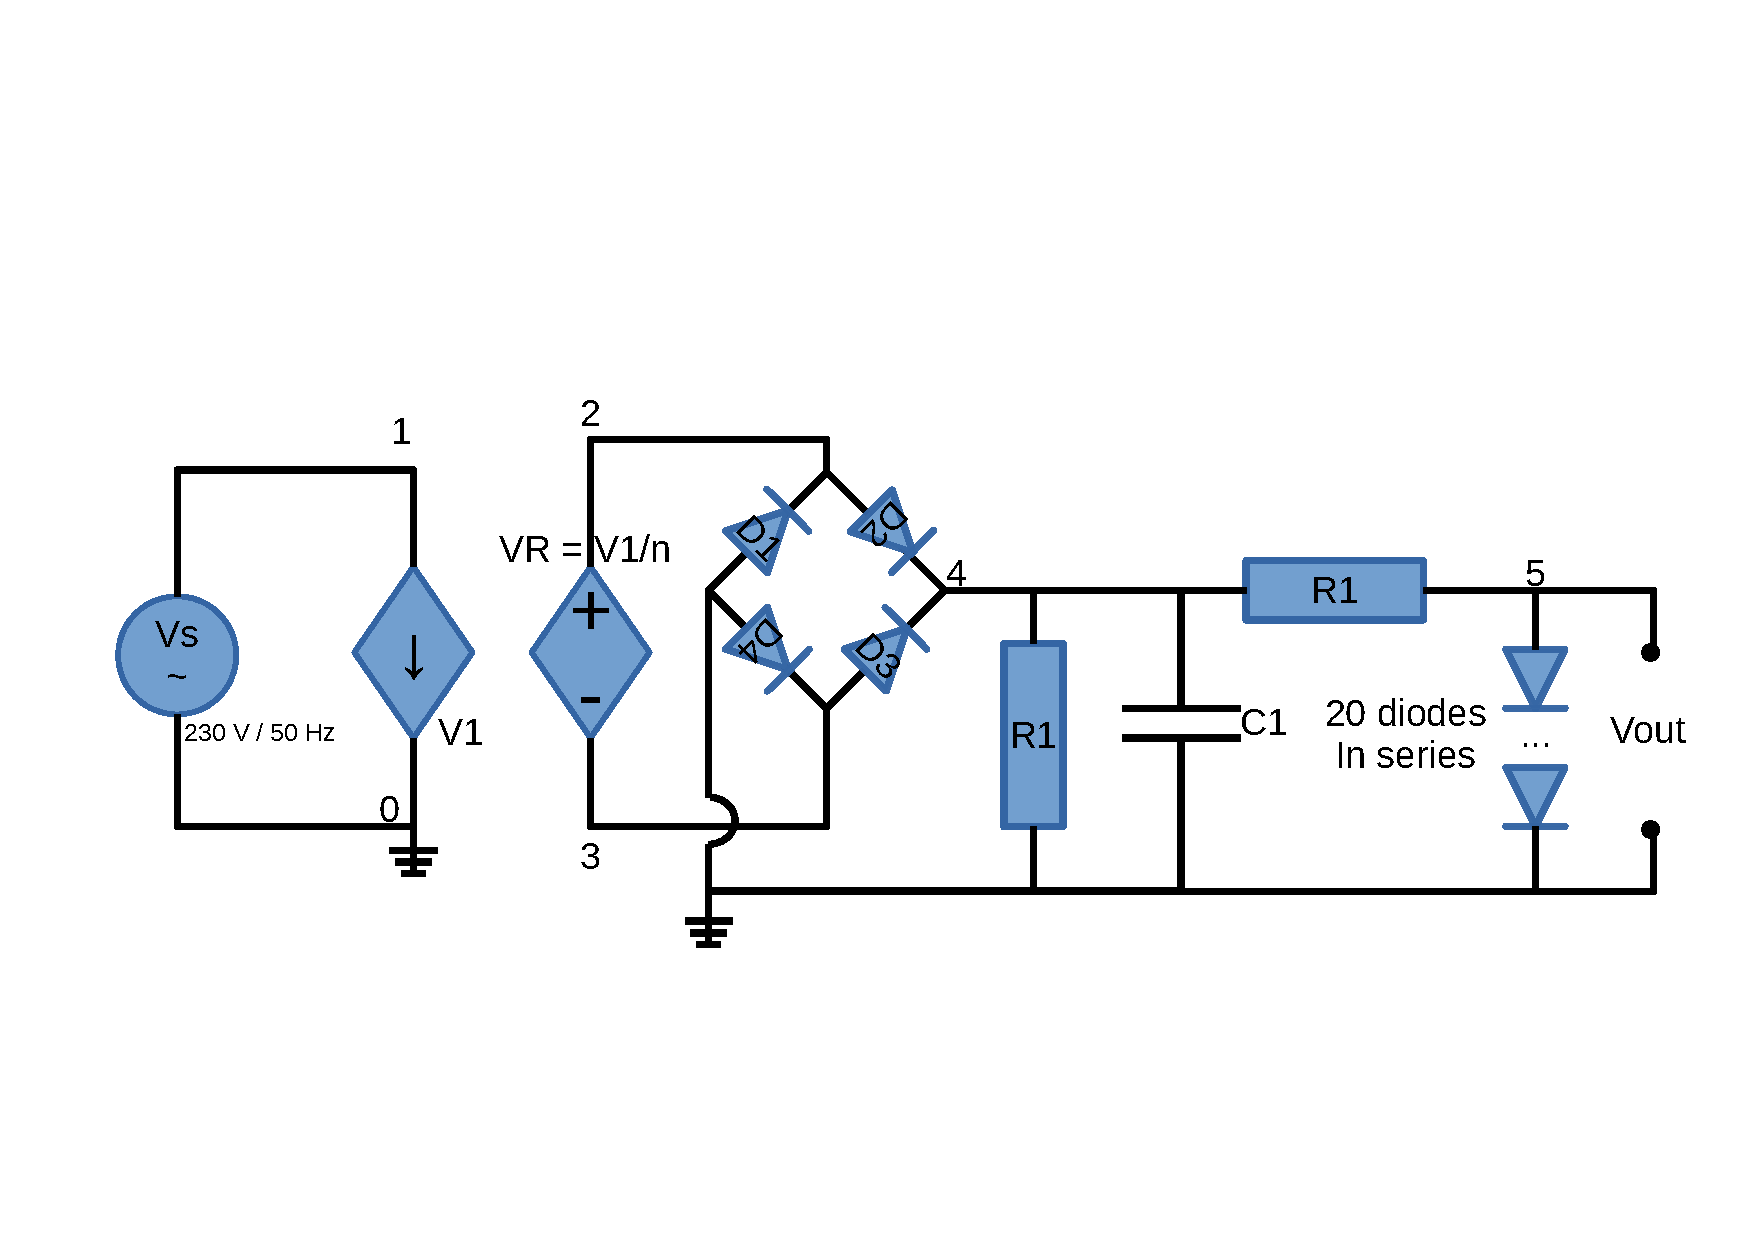
\includegraphics[width=0.7\linewidth]{./cir.pdf}
\caption{The AC/DC converter on which this report is based}
\label{fig:cir}
\end{figure}

\clearpage



\section{Theoretical Analysis}
\label{sec:analysis}
\subsection{Circuit frequency response}
With the equations below we determined the cut-off frequencies for the higher and lower cut-off frequencies. The former appears from the low-pass stage and the latter from the high pass stage.

\begin{equation}
w_L=\frac{1}{R_{1}C_{1}}
\end{equation}
\begin{equation}
w_H=\frac{1}{R_{2}C_{2}}
\end{equation}
This was the definition used to determine the central frequency, which is meant to be 1 kHz.
\begin{equation}
w_O=\sqrt{w_{H}w_{L}}
\end{equation}

\begin{table}[h!]
  \centering
  \begin{tabular}{|l|r|}
    \hline    
    {\bf Name} & {\bf Values} \\ \hline
    Lower Cut-Off Frequency & 723.431560 Hz \\ \hline 
Upper Cut-Off Frequency & 1446.863119 Hz \\ \hline 
Central Frequency & 1023.086723 Hz \\ \hline 
 
  \end{tabular}
  \caption{Cut off frequencies and central frequency.}
  \label{tab:data}
\end{table}

This central frequency result represents a 2.309\% relative error, which isn't a bad result considering the components used.

\begin{figure}[h!] \centering
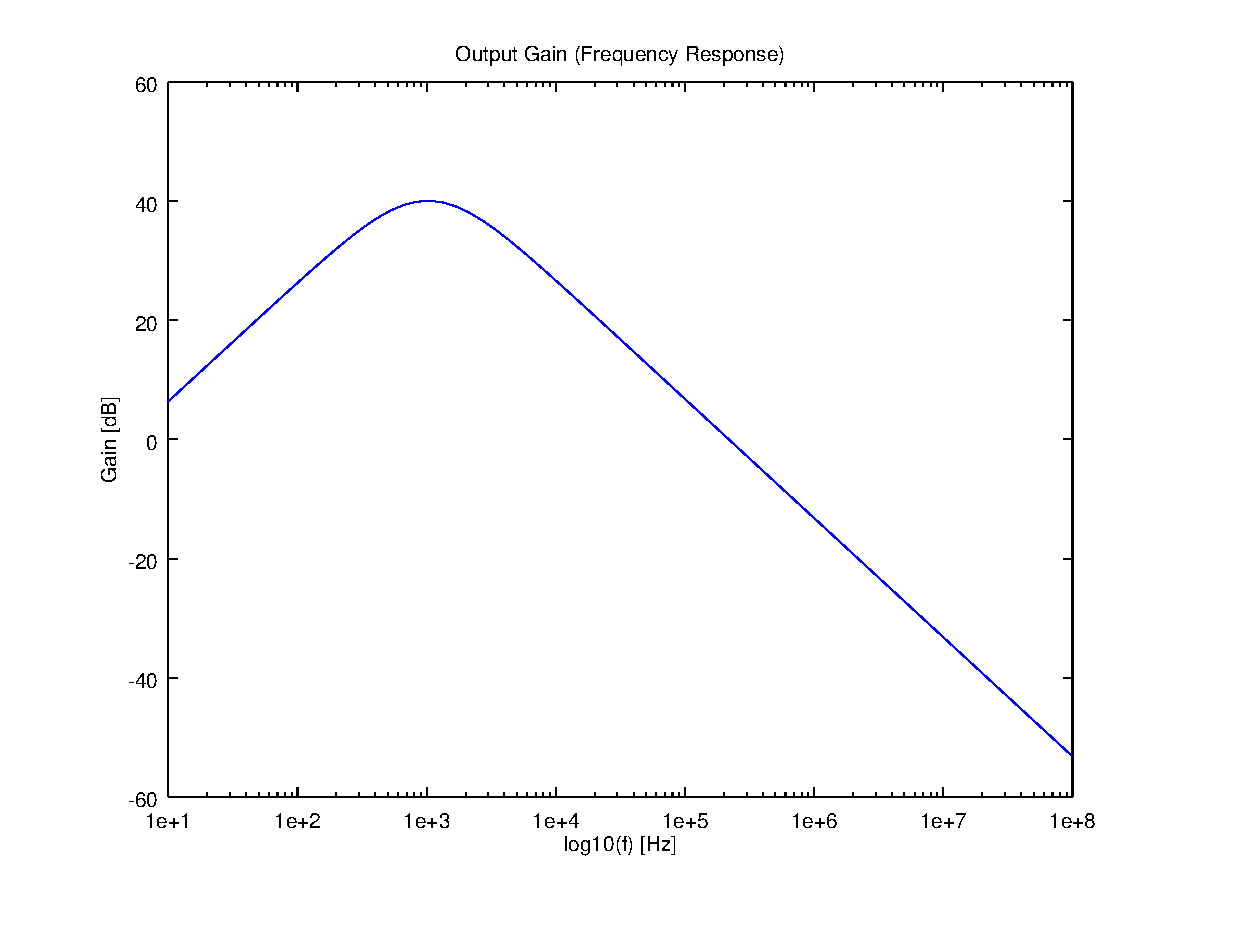
\includegraphics[width=0.6\linewidth]{gain.eps}
\caption{Voltage gain frequency response.}
\label{fig:gainfreq}
\end{figure}

As wanted, the plot has the trait of a narrower band-pass filter, with its top gain arriving in the 1 kHz neighbourhood, and the gain itself is on the 40 dB as pretended.

\begin{figure}[h!] \centering
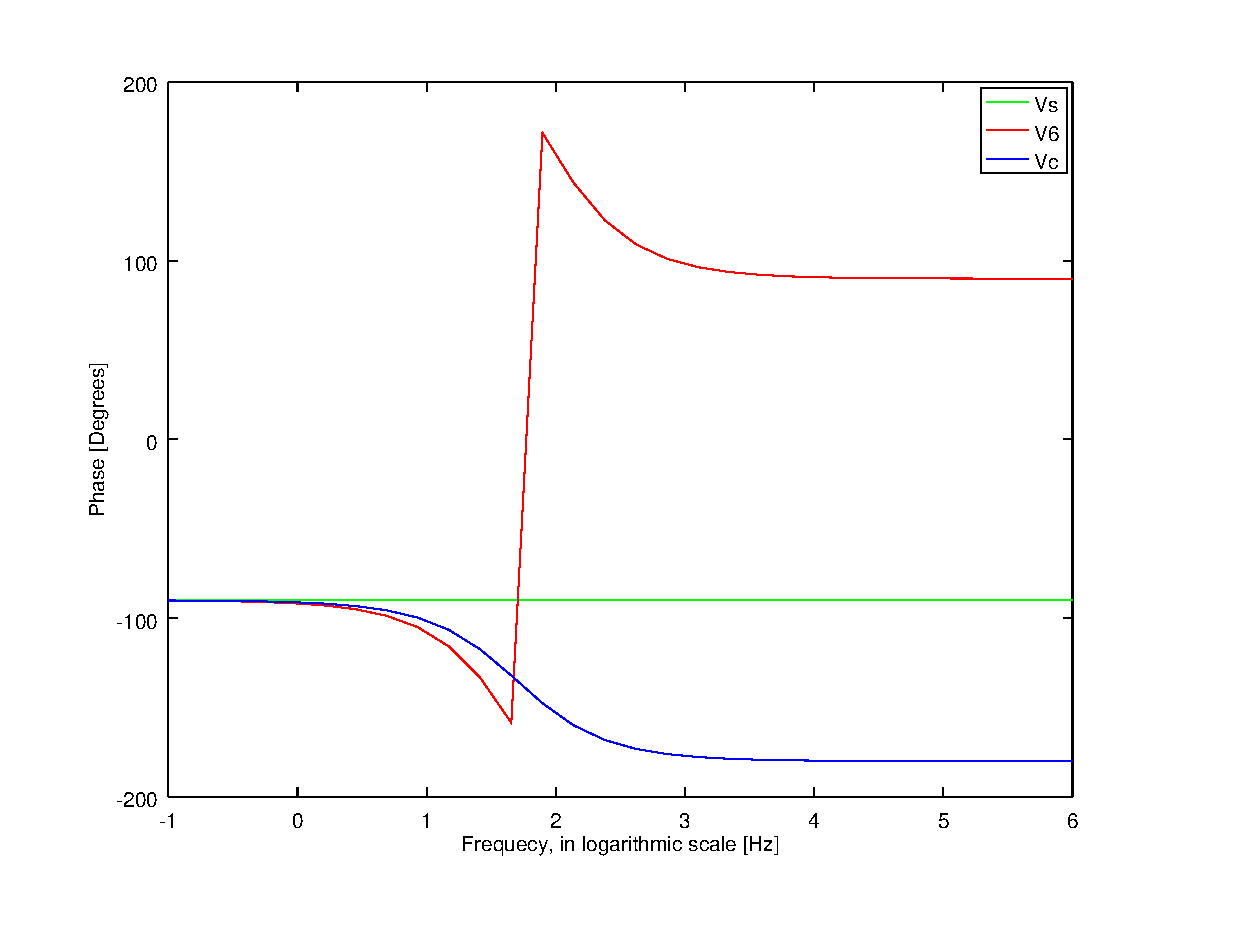
\includegraphics[width=0.6\linewidth]{phase.eps}
\caption{Voltage phase frequency response.}
\label{fig:gainfreq}
\end{figure}

The phase drops from 90 degrees to -90 degrees, which is cause of the 2 poles of the transfer function (which we will present in the next subsection), one pole introduced by the high-pass and the 
other pole introduced by the low pass. Each pole causes a 90 degree drop, 45º the decade before and 45º the decade after. At the central frequency, the phase is zero, which means the output 
voltage is in phase with the input voltage.

\subsection{Central frequency results}
For a frequency of 1 KHz we computed the circuit gain and input and output impedances for the amplifier. Also, we determined a theoretical figure of merit based on the predicted results with the set 
of values we chose.

The gain value for the entire circuit is obtained by multiplying the individual gains of each of the three stages of the circuit. This is an ideal situation, where we don't take into account the loss of signal between stages, or charge effects between the same stages.
These are the equations for the gain values:
\begin{equation}
High Pass Gain=|\frac{R_{1}C_{1}jw_{O}}{1+R_{1}C_{1}jw_{O}}|
\end{equation}
\begin{equation}
Amplifier Gain=1+\frac{R_{4}}{R_{3}}
\end{equation}
\begin{equation}
Low Pass Gain=|\frac{1}{1+R_{2}C_{2}jw_{O}}|
\end{equation}

Using the incremental model for the circuit (the input impedance of the OP-AMP is infinite and the output impedance of the OP-AMP is null, according to the model studied in class), we determined the following equations for the input and output impedances of the circuit:

\begin{equation}
Z_i = R_1 + \frac{1}{jw_{O}C_{1}}
\end{equation}
\begin{equation}
Z_o = \frac{R_2}{1+jw_OR_2C_2}
\end{equation}

\begin{table}[h!]
  \centering
  \begin{tabular}{|l|r|}
    \hline    
    {\bf Name} & {\bf Values} \\ \hline
    Gain (1 KHz) & 100.643363 \\ \hline 
Gain (1 KHz)(dB) & 40.055703 dB \\ \hline 
Gain (calculated central frequency) (dB) & 40.057714 dB \\ \hline 
$Z_{in}$ & 1000.000000 -723.431560j Ohm \\ \hline 
$Z_{in}$ modulus & 1234.241962 Ohm \\ \hline 
$Z_{in}$ phase & -35.883164 Degrees \\ \hline 
$Z_{out}$ & 676.732451 -467.723894j Ohm \\ \hline 
$Z_{out}$ modulus & 822.637497 Ohm \\ \hline 
$Z_{out}$ phase & -34.650304 Degrees \\ \hline 
Cost & 13626.952040MU \\ \hline 
Merit & 3.092445$*10^{-6}$ \\ \hline 
 
  \end{tabular}
  \caption{Gain, input and output impedances at the central frequency.}
  \label{tab:data}
\end{table}

This way we can see that the gain for a frequency of 1KHz is almost the same as the gain for the calculated central frequency, meaning the 1KHz frequency is still very much within the band pass region.
We obtained then a relative error of 0.643\% for the gain at central frequency, which is meant to be 100, so this a 
fantastic theoretical result. The input impedance value is quite high, which is good, so, depending on the resistance of the input, most of the input 
voltage will flow through ahead to the OP-AMP as pretended. The output impedance value though is quite large, so this circuit will not be suited to loads with very low resistance values, but given 
the components we had available there wasn't much room for improvement. Also, we don't know the load that would be linked to this circuit, so we can't fully know how good or bad this value is, 
we just know it is clearly not the most desirable.

\section{Simulation Analysis}
\label{sec:simulation}

In this section, the circuit shown in Figure~\ref{fig:rc} is simulated with the use of NGSpice. Using the operating point analysis for both $t<0~s$ and $t=0~s$, we determine the initial conditions needed for the transient analysis, which in turn simulates the circuit's total response.
Because of the use of NGSpice for this simulation, there was a need to create a "dummy" voltage source, between nodes 7 and 8, that provided $0~V$ to the circuit (thus not changing the behavior of the original circuit). Because this is just a technical issue that does not affect the original circuit, the one shown in Figure~\ref{fig:rc} can be used for illustrative purposes.


\subsection{Operating Point Analysis}

Table~\ref{tab:op} shows the simulated operating point results for $t<0~s$, where it's assumed that no current flows through the capacitor (open circuit).
Table~\ref{tab:op2} shows the simulated operating point results for $t=0~s$, where $V_S$ is short-circuited and the capacitor is replaced with a voltage source $V_x = V(6) - V(8)$ (with $V(6)$ and $V(8)$ as obtained in Table~\ref{tab:op}.


\begin{table}[h]
	\parbox{.45\linewidth}{
  \centering
  \begin{tabular}{|l|r|}
    \hline    
    {\bf Name} & {\bf Value [A or V]} \\ \hline
    v(1) & 5.048640e+00\\ \hline
v(2) & 4.860629e+00\\ \hline
v(3) & 4.468710e+00\\ \hline
v(4) & 4.888344e+00\\ \hline
v(5) & 8.679973e+00\\ \hline
v(6) & -2.02627e+00\\ \hline
v(7) & -3.01571e+00\\ \hline
v(8) & -3.01571e+00\\ \hline

  \end{tabular}
  \caption{Operating point data for $t<0~s$. A variable preceded by @ is of type Current and is expressed in Ampere; other variables are of type Voltage and are expressed in Volt.}
  \label{tab:op}
}
\hfill
	\parbox{.45\linewidth}{
  \centering
  \begin{tabular}{|l|r|}
    \hline    
    {\bf Name} & {\bf Value [A or V]} \\ \hline
    v(1) & 5.048640e+00\\ \hline
v(2) & 4.860629e+00\\ \hline
v(3) & 4.468710e+00\\ \hline
v(4) & 4.888344e+00\\ \hline
v(5) & 8.679973e+00\\ \hline
v(6) & -2.02627e+00\\ \hline
v(7) & -3.01571e+00\\ \hline
v(8) & -3.01571e+00\\ \hline

  \end{tabular}
  \caption{Operating point data for $t=0~s$. A variable preceded by @ is of type Current and is expressed in Ampere; other variables are of type Voltage and are expressed in Volt.}
  \label{tab:op2}
}	
\end{table}
            

\par Compared to the theoretical analysis results, one notices that the simulated data matches almost perfectly the theoretical values. This is expected, as the circuits being simulated in both scenarios are exclusively composed by linear components. Moreover, the slight discrepancies (of the order of $1e-15$) can be associated to the precision of ngspice and to some approximations made by octave because of the precision of the floating point used.

\newpage
\subsection{Transient Analysis}

\subsubsection{Natural Response}

Figure~\ref{fig:trans} shows the plot of the simulated transient analysis results in the interval $[0, 20]~ms$, using the boundary conditions of $V(6)$ and $V(8)$ as determined before. 
Once again, the simulation data matches with the theoretical natural response prediction, and one can clearly see the negative exponential behavior of $V(6)$, as was expected.

\begin{figure}[h] \centering
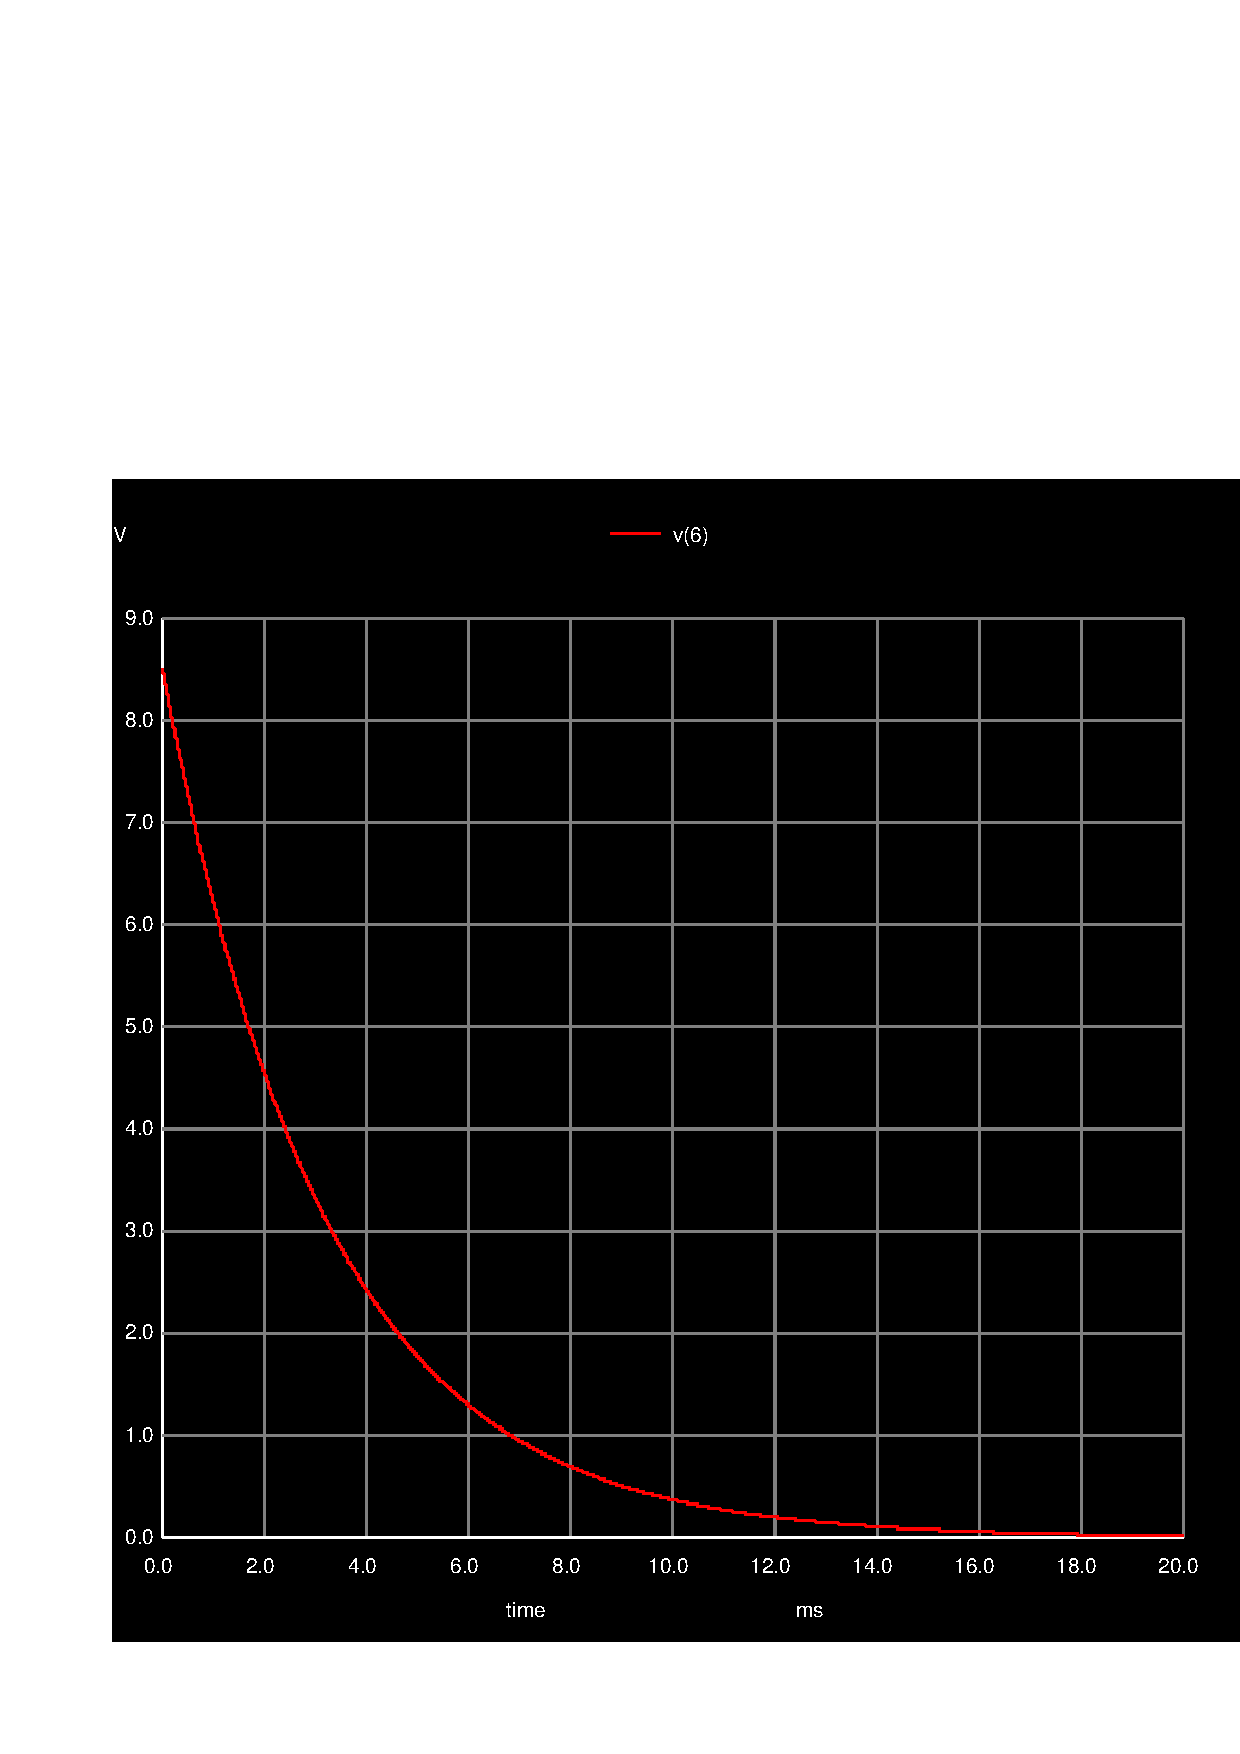
\includegraphics[width=0.6\linewidth]{natural.pdf}
\caption{Natural response of $V_{6}$ in the interval $[0, 20]~ms$.}
\label{fig:trans}
\end{figure}

\newpage

\subsubsection{Total Response}

Figure~\ref{fig:totalsim} shows the plot of the simulated transient analysis results in the interval $[0, 20]~ms$, by using $V_S(t)$ as given in Figure~\ref{fig:rc} and $f = 1~kHz$. 
Once again, the simulation data matches with the theoretical total response prediction, as was expected.
                                    

\begin{figure}[h] \centering
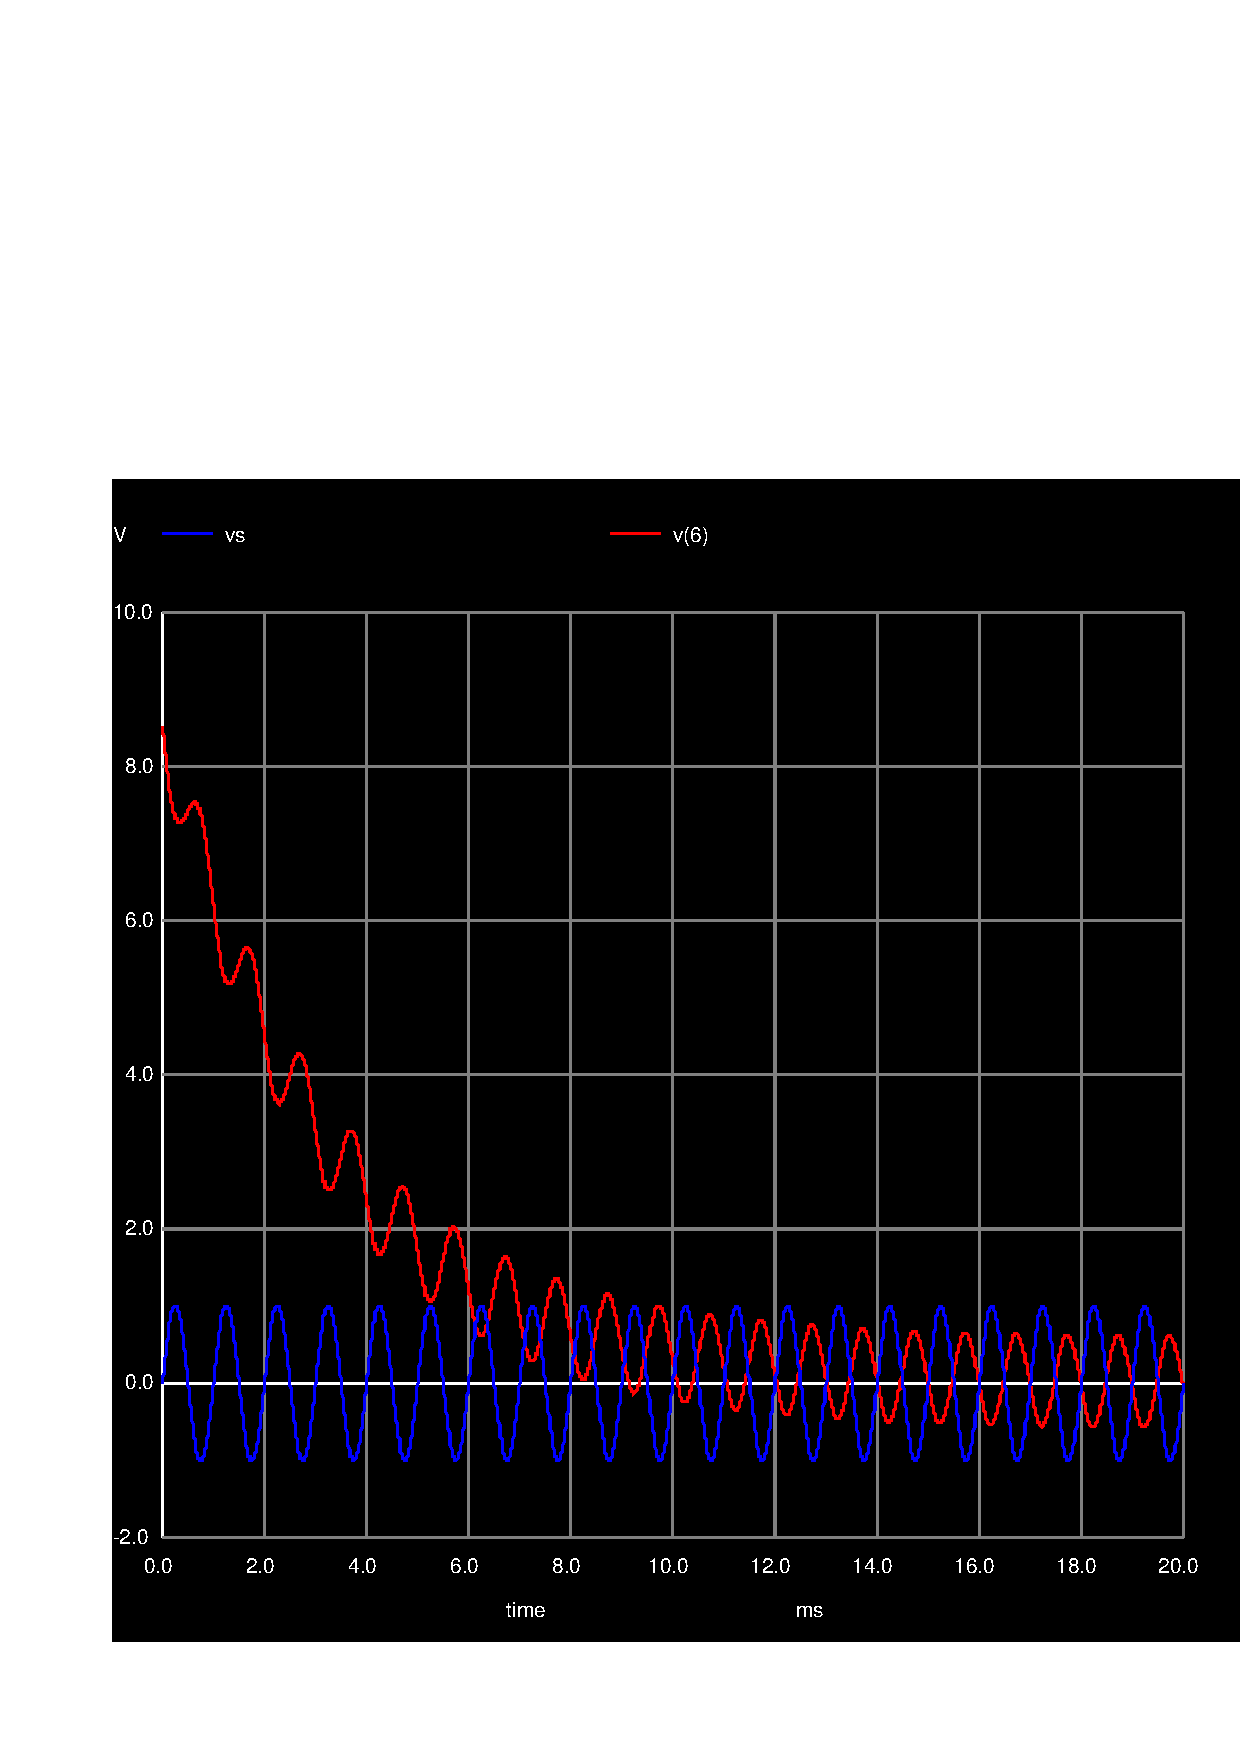
\includegraphics[width=0.6\linewidth]{total.pdf}
\caption{Total response of $V_{6}$ and $V_S$ in the interval $[0, 20]~ms$.}
\label{fig:totalsim}
\end{figure}

\newpage

\subsection{Frequency Analysis}

In this section, the frequency response in node 6 is simulated, with the frequency in logscale, magnitude in $dB$ and phase in $degrees$, for the frequency range of $0.1~Hz$ to $1~MHz$.


\subsubsection{Magnitude Response}

Figure~\ref{fig:magsim} shows the magnitude of the frequency response for the circuit under analysis. Compared to the theoretical analysis results, one notices a clear match between plots. Thus, the reasons for how $V(6)$ and $V_S$ differ from each other are the same as explained in the theoretical analysis above.

\begin{figure}[h] \centering
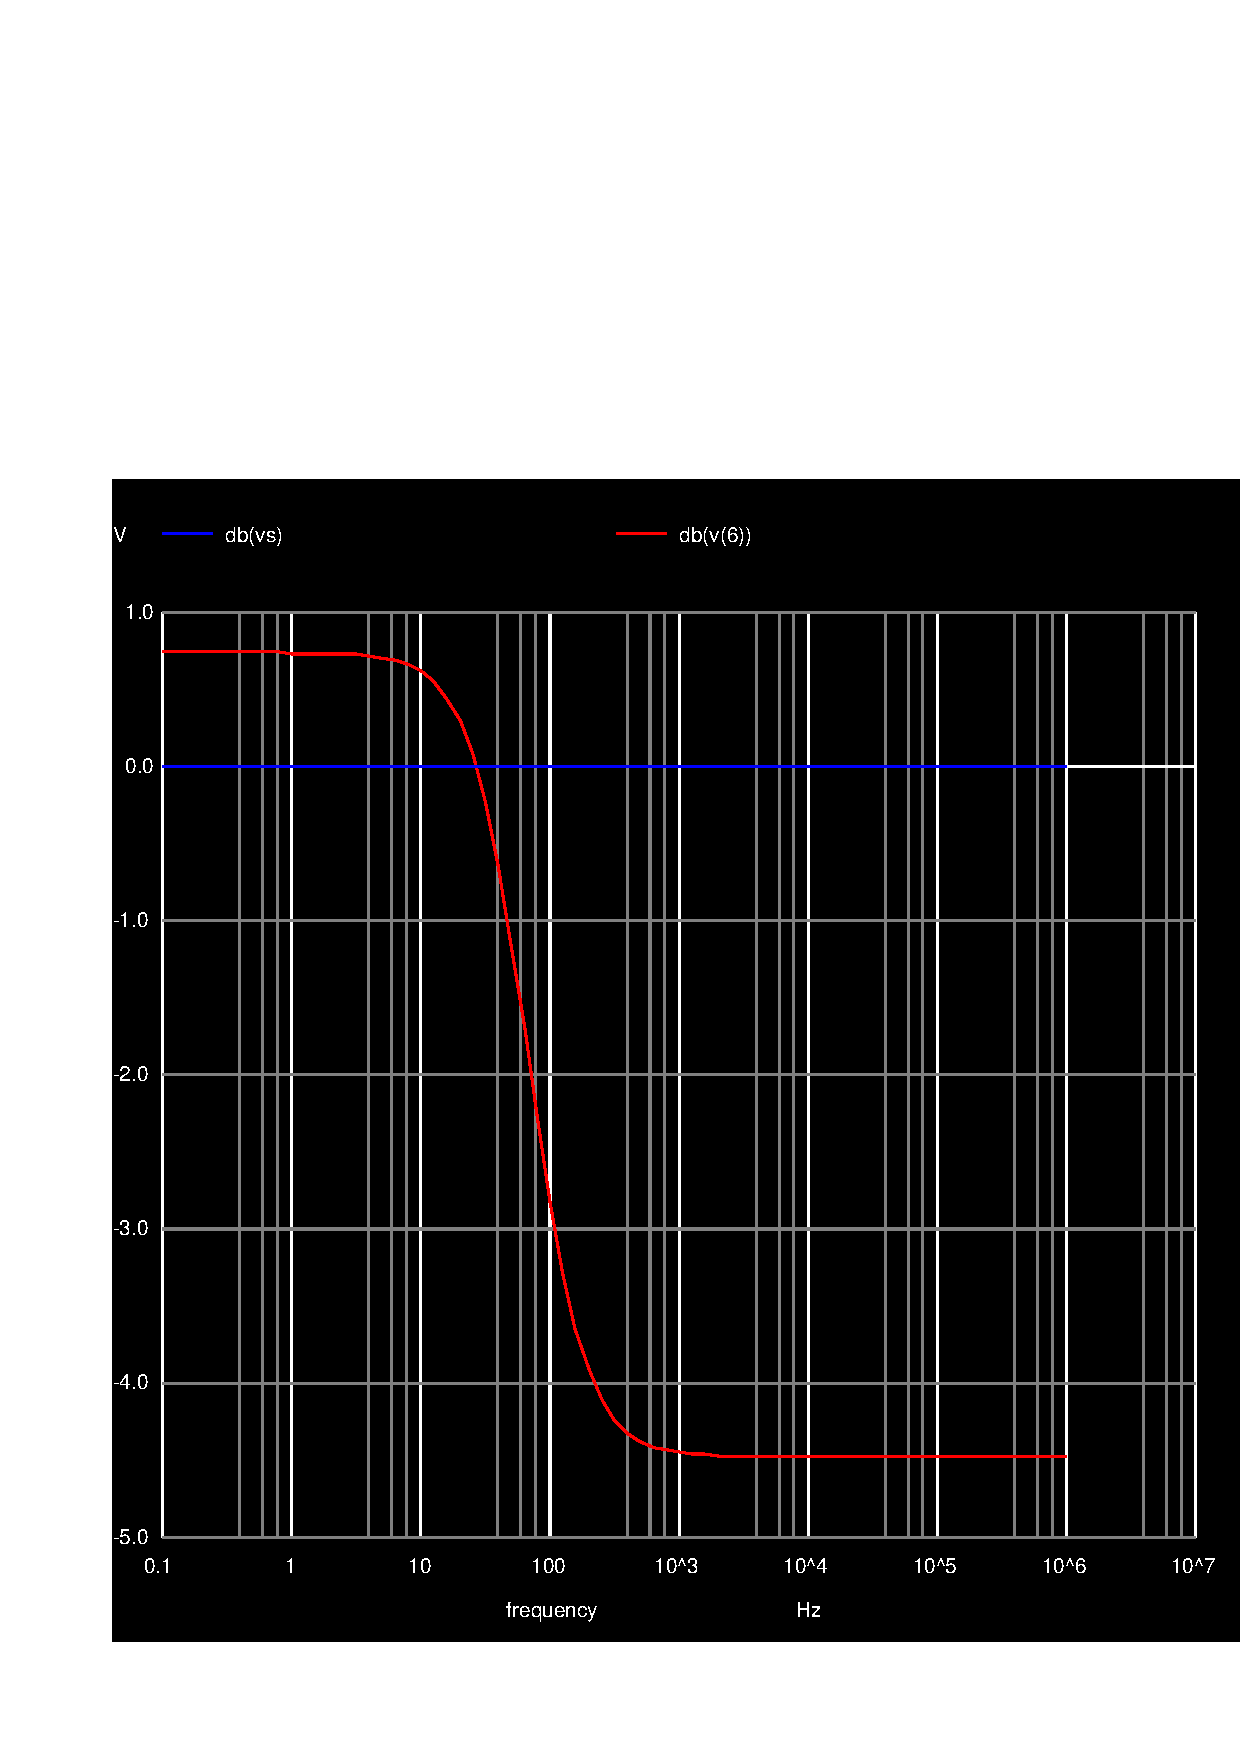
\includegraphics[width=0.6\linewidth]{magnitude.pdf}
	\caption{Magnitude of frequency response of $V(6)$ and $V_S$ plot.}
\label{fig:magsim}
\end{figure}

\newpage

\subsubsection{Phase Response}

Figure~\ref{fig:phasesim} shows the magnitude of the frequency response for the circuit under analysis. Compared to the theoretical analysis results, one notices a clear match between plots. Thus, the reasons for how $V(6)$ and $V_S$ differ from each other are the same as explained in the theoretical analysis above.

\begin{figure}[h] \centering
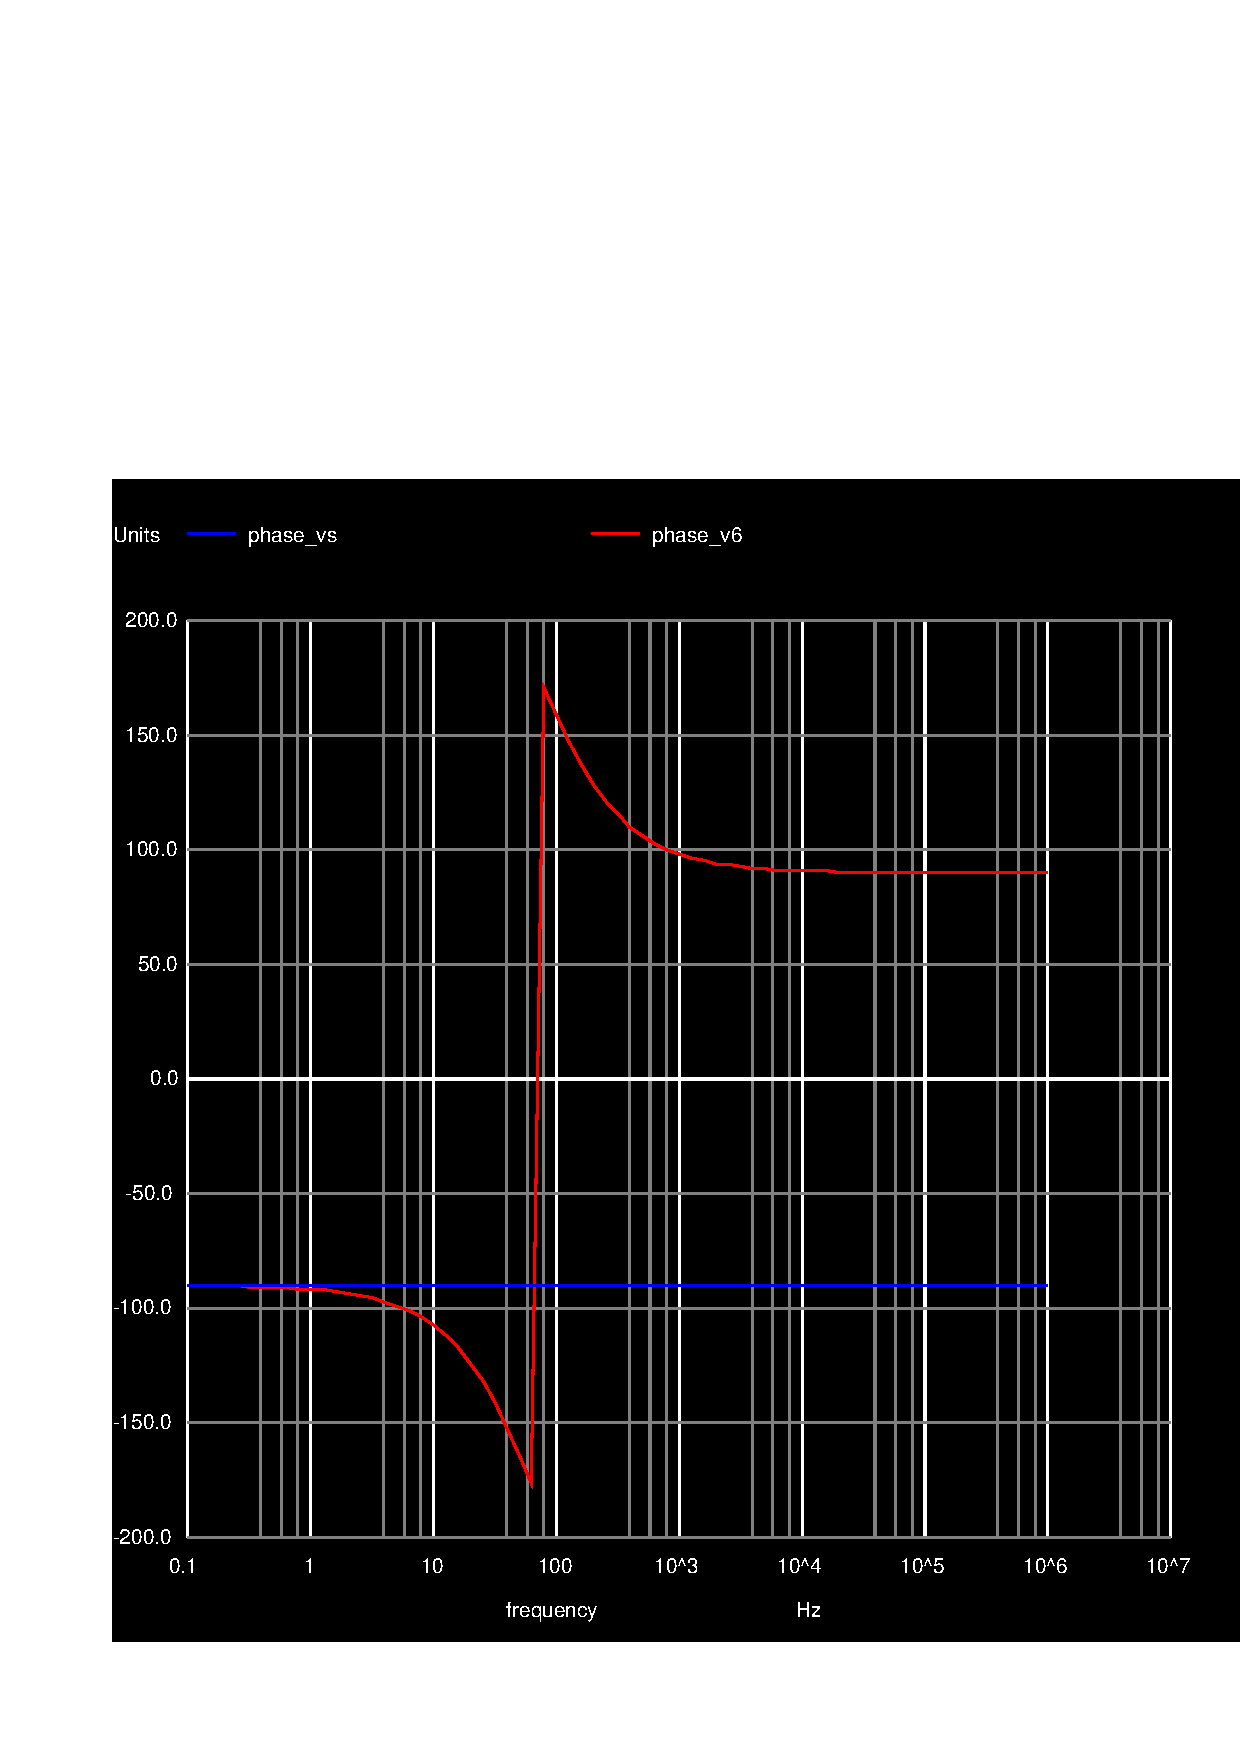
\includegraphics[width=0.6\linewidth]{phase.pdf}
	\caption{Phase response of $V(6)$ and $V_S$ plot.}
\label{fig:phasesim}
\end{figure}



\section{Conclusion}
\label{sec:conclusion}

\paragraph{} In this laboratory assignment the objective of creating and analysing an Audio Amplifier has been achieved with success. 
We have performed theoreticall and simulation analysis, using the Octave for the former and Ngspice for the latter.

\paragraph{} We found some discrepancies between both sets of results, which can be atributed, among other things, the fact that the circuit 
does not start from equilibrium. The fact that the impedance was high made this more evident. While these discrepancies are not ideal, specially 
for real world aplications, they can be expected and were mitigated.

\paragraph{} The table bellow has the Theoretical and Simulation results, allowing for it's comparison.

\begin{table}[!h]
  \centering
  \begin{tabular}{c c c c}
    \hline    
    {\bf Theoretical} & {\bf Value} & {\bf Simulation} & {\bf Value}\\ \hline
    Frequency response and impedances &  &  &  \\ \hline
$Gain$ & 100.643363 & Gain & 99.7361\\ \hline
$Gain(dB)$ & 40.055703 dB & Gain(dB) & 39.977 dB\\ \hline
$LowerCut-offFreq$ & 723.431560 Hz & Lower cut-off freq & 403.611 Hz\\ \hline
$UpperCut-offFreq$ & 1446.863119 Hz & Upper cut-off freq & 2386.17 Hz\\ \hline
$CentralFreq$ & 1023.086723 Hz & Central freq & 981.37 Hz\\ \hline
$Z_{in} Modulus$ & 1234.241962 Ohm & Zin modulus & 1.23431 kOhm\\ \hline
$Z_{in} Phase$ & -35.883164 Degrees & Zin phase & -35.8894 Degrees\\ \hline
$Z_{out} Modulus$ & 822.637497 Ohm & Zout modulus & 0.826194 kOhm\\ \hline
$Z_{out} Phase$ & -34.650304 Degrees & Zout phase & -34.3981 Degrees\\ \hline
$Cost$ & 13626.952040 & Cost & 1.362695e+04\\ \hline
$Merit$ & 3.092445*$10^{-6}$ & Merit & 3.883972e-06\\ \hline
 
  \end{tabular}
  \caption{Comparison of the theoretical and simulated data results, regarding the operating point, frequency response and impedances.}
  \label{tab:comp}
\end{table}

\paragraph{} We also believe that, given the satisfactory results obtained by us, the model used could be applied in a real life Audio Amplifier.

\paragraph{} Finally, this assignment allowed us to gain some further knowledge in the application of the subjects topics.








%\cleardoublepage

% ----------------------------------------------------------------------
%  Bibliography
% ----------------------------------------------------------------------
%\addcontentsline{toc}{section}{\bibname}
%\bibliographystyle{abbrvunsrtnat} % <<<<< SELECT IF USING REFERENCES BY NUMBER (CITATION ORDER)
%\bibliography{../../../BIBfile.bib}

% ----------------------------------------------------------------------
\end{document}
% ----------------------------------------------------------------------
